\restoregeometry

\cxset{
 name={CHAPTER},
 numbering=arabic,
 number font-size=\Large,
 number font-family=\rmfamily,
 number font-weight=\normalfont,
 number before=\kern0.5em,
 number after=\hfill\hfill\par\vspace*{20pt}\centerline{\decoone}\vspace*{20pt},
 number dot={},
 number position=rightname,
 name=CHAPTER,
 chapter font-family=rmfamily,
 chapter font-weight=mdweight,
 chapter font-size=Large,
 chapter before={\vspace*{20pt}\par\hfill},
 chapter after={},
 chapter color=black!90,
 number color=black!90,
 chapter title align=center,
 chapter title text-align=center,
 title margin-left=0pt,
 title margin bottom=50pt,
 title margin top=30pt,
 title before=,
 title after=,
 title font-family=rmfamily,
 title font-shape=upshape,
 title font-color= black!90,
 title font-weight=\normalfont,
 title font-size=Huge,
 title display=block}

\chapter[Style 18]{Chapter Style Eighteen}

\parindent0pt
This design introduces an ornament. There are a number of packages on ctan that provide ornaments. If you using XeLaTeX it is also possible to use system fonts. The ornament is introduced with the key number after. At this point also we introduced all the vertical skips.
\medskip
\begin{figure}[ht]
\centering
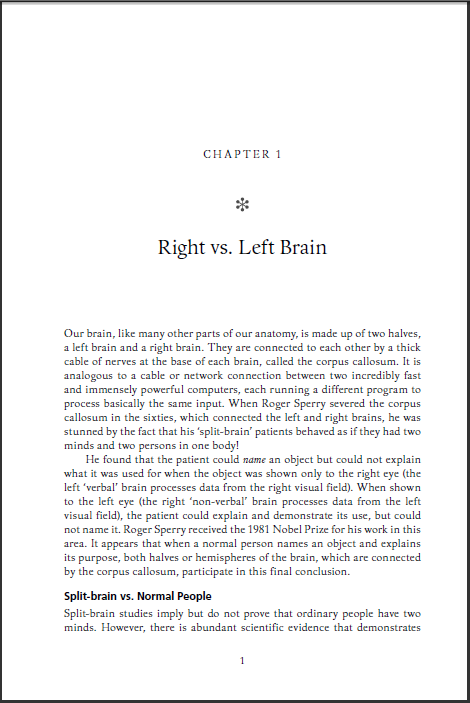
\includegraphics[width=0.45\textwidth]{./chapters/chapter18.png}
\end{figure}

\section{Sections}
\lorem

\subsection{Subsections}
\lorem


\subsubsection{Subsubsections}
\lorem

\parindent3em
\newcommand{\wb}[2]{\fontsize{#1}{#2}\usefont{U}{webo}{xl}{n}}
\newcommand{\showb}[1]{\wb{12}{14}#1}
\newfontfamily{\minion}{MinionPro-Regular.otf}
\def\ornament{{\minion \char"2740}}

\cxset{chapter name=,
          epigraph align=center,
          epigraph text align=center,
          epigraph rule width=0pt,
          title margin top=10pt,
          number font-size=small,
          number after=\hfill\hfill\par\vspace*{5pt}\centerline{\showb{[]}}\vspace*{5pt},
           %number after=\hfill\hfill\par\vspace*{5pt}\centerline{\Large\ornament}\vspace*{5pt},
          }
\chapter{THE IMPRESSIONISTS IN NEW YORK}


\epigraph{\ldots\itshape a pile of unsung treasures \ldots}{}
\minion

\lettrine{O}{n 13 March 1886, Paul Durant-Ruel and his young son Charles were travelling} through the streets of Paris, on their way to Gare Gare Saint-Lazare. In the two decades since Paul had
inherited his father’s business, Paris had been transformed. Haussmann had
realized his dream. The city was only three years away from the
Exposition of 1889 and the erection of the new Eiffel Tower, the symbol
of modern Paris. By 1890, Baron Haussmann would be saying of his newly
created capital of Europe, ‘these days, it’s fashionable to admire old Paris,
which people only know about from books’. Some areas of Paris had
hardly changed: the poor still lived in the shacks of Montmartre or the
shanties of Belleville; there were still cholera, typhoid, deaths in childbirth
and infant mortality. But to the uninitiated, those problems were now
hidden from view. Paris had a new image: the new Republic was
streamlined and stylish, the epitome of healthy living and good taste.
Haussmann’s Paris was architecturally modern, stratified by wealth,
quintessentially urban and, above all, commercially prosperous.

\begin{figure}[ht]
\centering
\fbox{%
\includegraphics[width=0.8\textwidth]{impressionist-lives}}
\caption{Spread from the Book \emph{The Private Lives of the Impressionists} by Sue Rose and published by Harper Collins.}
\end{figure}

The ctan repository has two good packages for ornamental fonts \pkgname{webomints} and \pkgname{fourier-orns}. The one shown in the orgininal publication is from Minion Symbols Pro.

They have been inserted in the template by using the |number after| key and a custom command from the \pkgname{webomints}
\bigskip

\begin{scriptexample}{}{}
\begin{verbatim}
\newcommand{\wb}[2]{\fontsize{#1}{#2}\usefont{U}{webo}{xl}{n}}
\newcommand{\showb}[1]{\wb{12}{14}#1}
\end{verbatim}
\end{scriptexample}


\ornament

\let\oldsection\section
\long\def\section{%
\par\medskip
\addvspace{20pt}
\centerline{{\LARGE *}}%
\addvspace{20pt}}


Cézanne wanted nothing to do with any war. Taking Hortense with him,
he left their garret at 53, rue Notre-Dame-des-Champs, and made for Aix.
Zola, who had recently married, returned to Provence with his wife,
heading from there to Marseilles. Monet, still in Trouville, waited for the
time being to see how events would turn out. Degas, Renoir, Bazille and
Manet, who stayed behind, were all eligible to fight

Cézanne had been working right up to the last minute to meet the 1866
Salon deadline. On the last possible day for submitting, a wheelbarrow
arrived outside the Palais de l’Industrie, pushed and pulled by Cézanne
and Oller, his Cuban friend from Suisse’s. Cézanne rushed to unwrap his
paintings, eager to show them to anyone who wanted to see. But by now
his hopes were not particularly high. When both his paintings were
rejected he was hardly surprised. He headed straight back to Aix,
complaining to Pissarro about the ‘rotten’ family he was being forced to
rejoin, all of them ‘boring beyond measure’. 

\section

Sections are marked with a single asterisk like ornament. This is a common element
in many non-fiction as well as fiction books. Some might have anything from on to three
asterisks. Many books printed in the nineteenth century have very fancy end section ornamentation.
I like the simplicity of the one asterisk.

\let\section\oldsection
\cxset{title display=in-line block}


